% !TeX spellcheck = en_US

\chapter{Git and GitHub}


%------------------------------------------------------------------------------------------------------
\section{Introducing Git}
    
Version Control Systems (VCS) are in charge of registering all the modifications made on a bunch of files, saving copies of the files, 
recording what changes have been made, at what time, by who, etc. 
The following actions can be carried out by a version control system such as Git: 

\begin{enumerate}
\setlength\itemsep{0.0cm}
    \item Old versions of the project can be recovered in the future.
    \item The evolution on the project can be tracked.
    \item It is easier to collaborate on the same project with a group of people.
    \item Incompatible or simultaneous changes in the same files can be managed by conflict resolution tools.
\end{enumerate}

Git is a software to track changes in computer files what makes it ideal for software development (individual and among groups). 
Once it is installed in the computer any project can be managed by Git, that project is then called repository.
When some project is tracked by Git, a \texttt{.git} hidden folder and some other files (i.e. the file \texttt{.gitignore}) appear in the 
repository.
The version control system can be used from the command prompt once \texttt{git} is installed. 
Those \texttt{git} commands can be also be invoked from graphical interfaces such as: Visual Studio, 
GitHub or GitHub Desktop. 

It is important to distinguish between the local repository (your personal computer) and the remote
repository such as GitHub.  
GitHub is a provider of Internet hosting for software development and version control using Git.
It is a web-based hosting service that allows to store files in the cloud in a private or public repository. 
The next sections covers the creation of local and remote repositories as well as 
procedures to work with collaborators and teams by developing software or modifying files. 


 
\section{Create a remote  GitHub repository}
 
 First of all, a GitHub account must be created to store remote repositories. 
 Go to \textit{github.com/join} and create a GitHub account associated to your email.
 There are different ways to create a remote repository depending on the graphical user 
 interface you use: 
   
 \begin{enumerate}
 \item {\bf From the GitHub web page.} Once our GitHub account has been created, login in the GitHub web page 
 with our credentials and click \textit{+} button close to your photo to create a repository. 
 Follow the steps to create the basic files of the repository such as \texttt{.gitignore} file,  
 and \texttt{README.md} file to start with. 
   
 \item {\bf From Visual Studio. } 
 Open some Visual Studio project that you are working with. 
Click on \textit{GIT/Create Git Repository}, 
 select the GitHub account, choose the repository name and create and push.
Browse through your  GitHub web page to see your new repository. 
 
 \item {\bf From GitHub Desktop. }
  Open GitHub Desktop and sign in with your GitHub account 
  (\textit{File/Options/Accounts}).  
  Create a new repository (\textit{File/New repository}) by selecting its name, 
  a \texttt{REAMDE.md} file and a \texttt{.gitignore} template. 
  Click on \textit{Create repository} and then \textit{Publish repository}.
  Browse through your GitHub web page to see your new repository.
  \end{enumerate} 



\section{Clone a remote repository}

There are three different ways to clone a remote repository 
so a local repository is created. 
Go to any GitHub public repository and from the green button  \textit{Code}
click on: 
 \begin{enumerate}
 \item {\bf  Open with GitHub Desktop.}
 This option opens the GitHub Desktop application and allows to select the  
 local path where this repository will be stored. 
  Click on \textit{Clone} to create the local repository. 
 \item {\bf  Open with Visual Studio. } 
 This option opens Visual Studio and allows to select the local path where this repository 
  will be stored. Click on \textit{Clone} to create the local repository. 
 \item {\bf Download zip. } 
 This option downloads a zip file that can be decompressed in any selected folder.
  
\end{enumerate} 



\section{Workflow and nomenclature in Git}
Before dealing with the recommended workflow to work with Git, it is important
to define nomenclature  and important concepts to understand the proposed protocol.
These concepts are  shown graphically in figure \ref{fig:WorFlowGit}. 
Once files are under \texttt{Git}, they are \texttt{TRACKED} which means that their 
modifications are registered every time a \texttt{COMMIT} is performed. 
Once theses changes are validated, they are uploaded to the cloud by a \texttt{PUSH}  
order. On the other hand, 
when the most recent version of the remote repository is needed, a \texttt{PULL}  
order will allow to download  files from the remote repository to the local repository.  


Sometimes, auxiliary or executable files do not need to be tracked because 
they are automatically generated from sources files and their changes depend only on the
source files. By that reason, those files are ignored by \texttt{Git} by specifying in the 
\texttt{.gitignore} their specific extension such as: \texttt{*.exe} or \texttt{*.aux}.  
   
    
\begin{figure}[h]
    \centering
    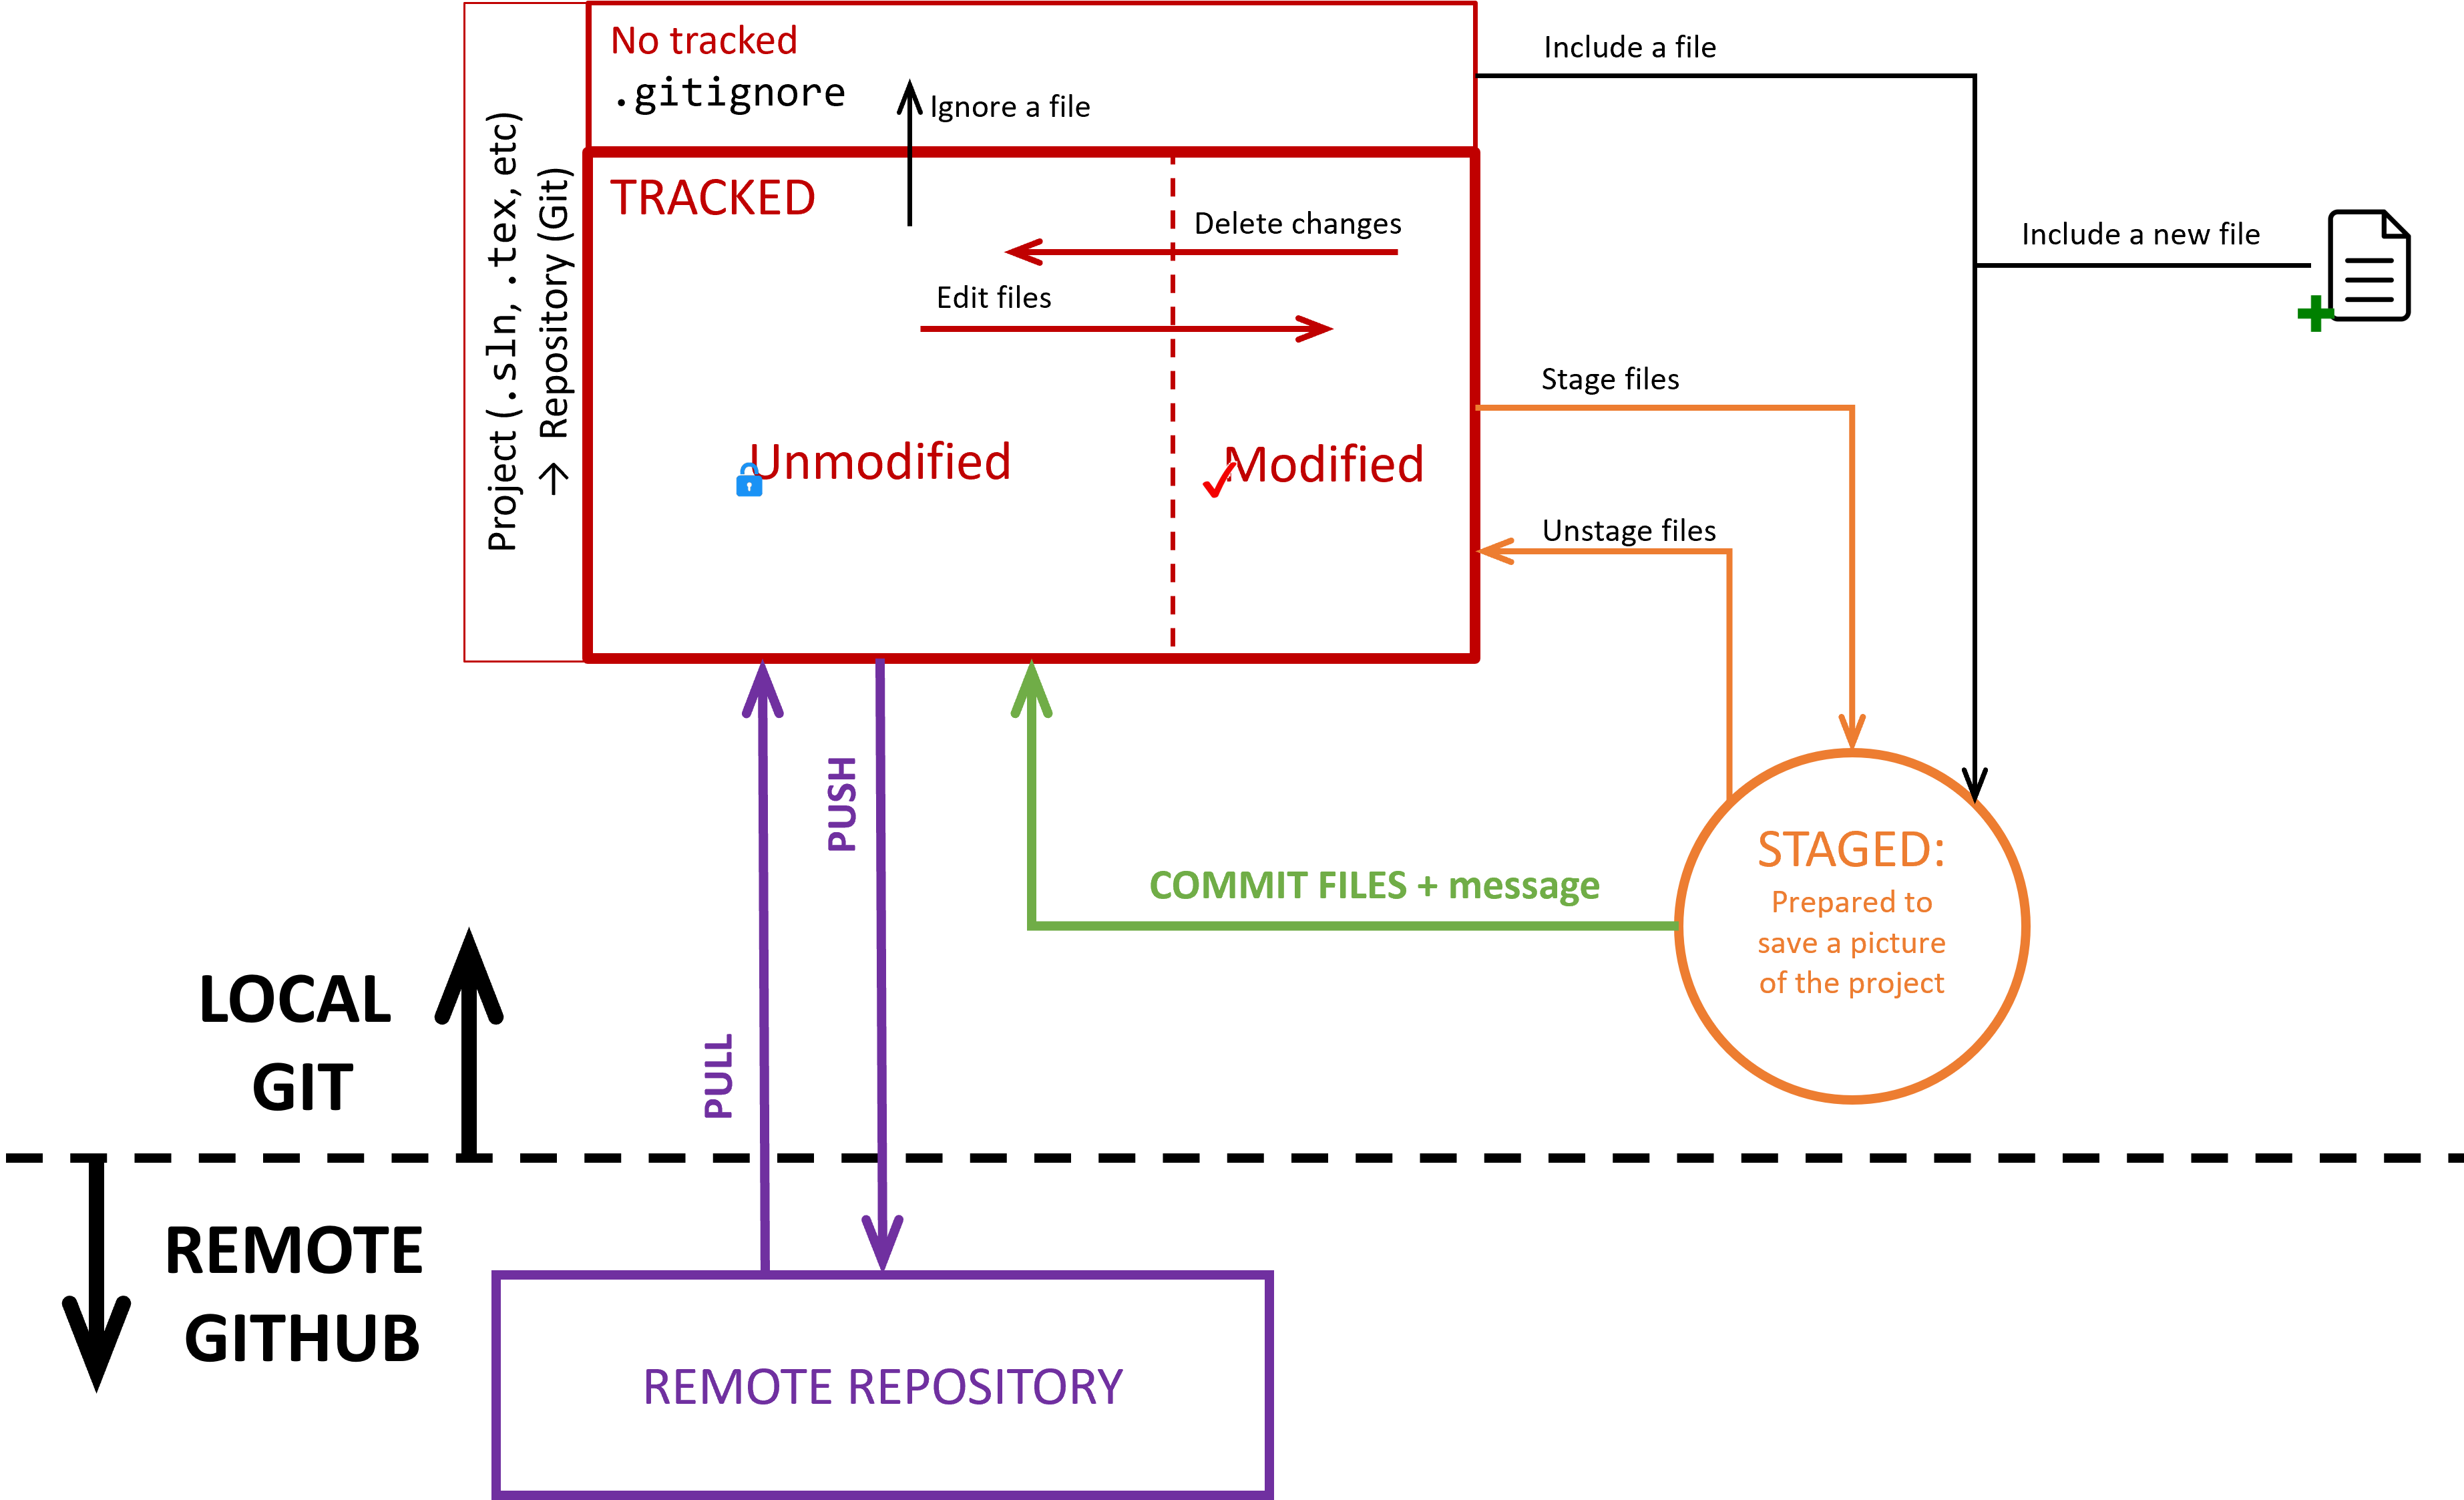
\includegraphics[width = \textwidth]{Figures/GHStates.png}
    \caption{Main states of Git and GitHub workflow.}
    \label{fig:GitStates}
\end{figure} 

\begin{figure}[h]
    \centering
    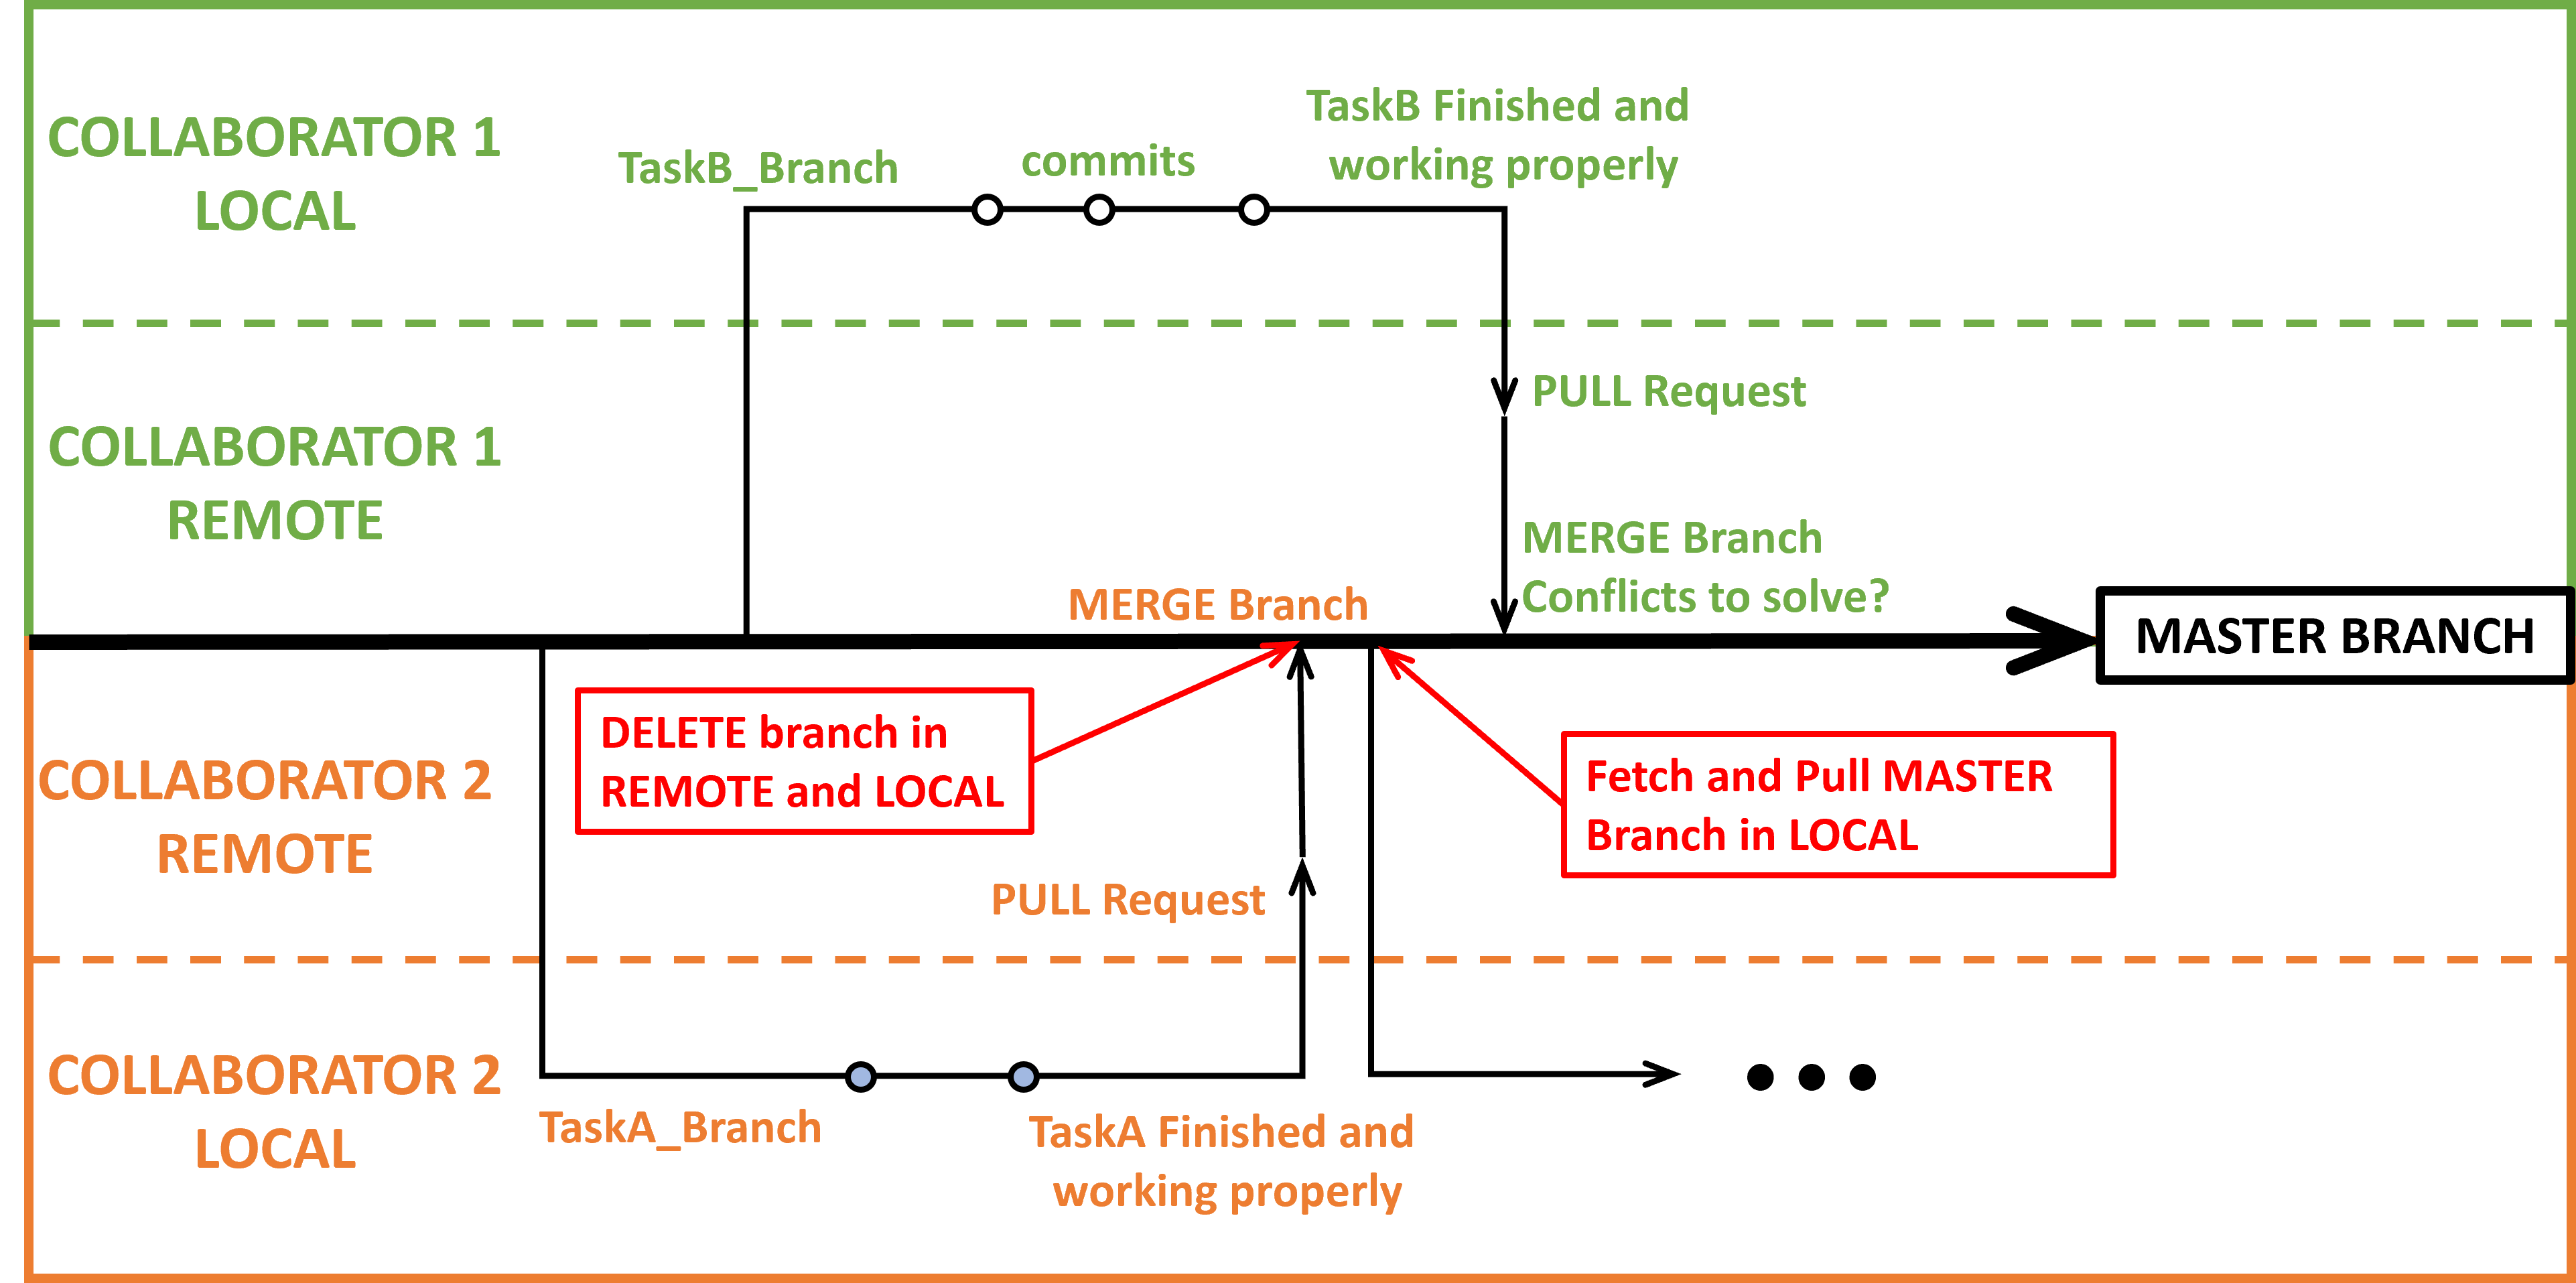
\includegraphics[width = \textwidth]{Figures/WorkFlowGit.png}
    \caption{Recommended Workflow when collaborating with GitHub.}
    \label{fig:WorFlowGit}
\end{figure} 
  



\section{How to work with Git}
Once a remote repository has been created, later improvements or modifications 
should be carried out with a pristine protocol in order to be efficient in developing
software. Some specific rules are proposed to define this protocol.
To modify some part of a software code, decide the name of the specific 
task you are going to deal with and create a new branch based on the newest version of 
the master branch. Even if you are the owner of the repository,
do not make changes in the master branch. 
Use your new branch to validate your changes. 
Once these changes are validated, try to merge this branch with the master branch to 
consolidate those changes.
The following procedure should be carried out: 
 \begin{enumerate}
 \item {\bf Modify}. Make changes of sources files, compile and test. 
 \item { \bf Commit changes}.  Once your changes are clear enough to solve or 
 improve your specific task, commit changes. 
 The frequency of different commits depend on the expertise of the programmer or developer 
 but it is always safer to increase the frequency of commits if you don't fell comfortable 
 with those changes.  
 \item {\bf Push changes}.
 Once a bunch of committed changes are validated, upload to changes to GitHub 
 with a push order. It allows to have the more recent version of your branch
 uploaded to GitHub if some collaborator want to check it or to give you feedback. 

 \end{enumerate}
If collaborators are going to work in some repository, the owner of the repository
could invite people to collaborate  (\textit{settings/manage access}).
Even if you are not invited to collaborate, you can create a fork of any public repository 
and to propose later a pull request.  
 
\section{How to merge two branches}
When the developer decides his task is finished and ready to be shared, 
he should merge his branch with the master branch. 
If only one person is  working  or 
if the developer is working only in one specific task at a time, 
no conflicts are going to arise when trying to merge different branches  
(notice at this point the importance of having the branch you work on
based on the most updated version of the main branch).
However, if two collaborators are modifying the same file, conflicts should be resolved. 
This process is shown graphically in figure \ref{fig:WorFlowGit} where two collaborators 
are working on two different branches or tasks.  
As it was mentioned before, it is a good practice not to modify the master branch 
and to create specific branches with a succinct label describing the purpose of the task or 
branch. The following steps represent the proposed methodology to work with collaborators:   
\begin{enumerate} 
\setlength\itemsep{0.0cm}
\item Collaborators 1 and 2 create branches  $b_1$ and  $b_2$ 
respectively based on the same master branch. 
\item Imagine that collaborator 2 
finishes his task before collaborator 1 and merges his branch $b_2 $  with the master 
branch. He will not find conflicts because no one has merged with the master branch after 
 branch $b_2$ was created. 
\item Imagine that collaborator 1 finishes his branch and tries to merge. 
If both collaborators are working on the same files, 
collaborator 1 could find conflicts when trying to merge branch $b_1$ with the master branch 
because at the time he tries to merge,  master branch is different from what 
it was previously based on. 
Hence, when working in teams possible conflicts could arise and they should be resolved. 
\end{enumerate} 
 
There are ways to merge and  to resolve possible conflicts of two different branches: {\it (i) } From GitHub and    
 {\it (ii) } From Visual Studio.  
%There are two ways to merge two branches to finish some specific task, 
%to resolve conflicts if they appear and to delete old branches. 

\section{Merging and resolving conflicts from GitHub} 
 From  from GitHub or Visual Studio
create a pull request to pull changes of some specific branch to be merged with the master branch. 
Now, from GitHub web page \textit{create the pull request} and \textit{merge} accepted changes
if no conflicts appear. 
If conflicts appear, GitHub allows to open with a web editor those files associated with 
conflicts. By deleting manually those parts of files which are not accepted, 
conflicts are resolved. Once this is done, \textit{Mark as resolved} to accept changes
by a \textit{Commit merge}.
The following steps  summarize the merging process, from GitHub, of two branches with conflicts:
 \begin{enumerate} 
 \setlength\itemsep{0.0cm}
 \item Create pull request 
 \item Open the web editor and solve conflicts.  
 \item Mark as resolved. 
 \item Commit merge. 
  \end{enumerate}  
  
  

\section{Merging and resolving conflicts from VS}

 Select \textit{Git/Manage branches} and from the master branch (it has to be active),  merge  
 by clicking on the specific branch with the right button and choose
 \textit{merge branch into master}.
 If conflicts appear click on \textit{Resolve conflicts} and then look for Git changes 
 where a list of files with changes with conflicts will appear.
 Click right button on each file and select {\bf merge}. Three windows will appear showing 
 the incoming modification file, the current master file and the desired result or merge file. 
 By selecting different ticks or differences between 
 the modification file and the master file, the result file is built. 
 Once you agree with the result file, click on {\bf Accept merge} and commit the merge. 
 The following steps  summarize the resolving process when merging two branches with conflicts:
 \begin{enumerate} 
 \setlength\itemsep{0.0cm}
 \item Select master branch. 
 \item Select \textit{Git/Manage branches}. 
 \item Click right button on the branch to merge and click on \textit{Merge this branch 
 into master branch}. 
 \item Click on \textit{Resolve conflicts} (in blue).
 \item Select \textit{Git changes} to identify a list of files with conflicts. 
 \item Click right button on the file presenting conflicts and select {\bf merge }.
 \item Select differences or ticks between the two branches to merge and validate the result. 
 \item Accept merge. 
 \item Commit the merge result. 
 \item Push to the remote repository. 
 \end{enumerate}

Once conflicts are resolved and some specific branch is merged with the master branch, 
it is mandatory  to delete the local and the remote specific branch which was used to work in this task. 
If a new modification is going to be carried out, 
a new branch should be created based on the most recent update of the master branch. 

\section{How to revert specific commits} 
There are three different stages from which modifications or changes  can be reverted: 
\begin{enumerate}
 \setlength\itemsep{0.0cm}
\item Before changes are committed. 
\item After changes are committed.
\end{enumerate}
If changes are not still committed, select \textit{Git changes} and a list of files that 
have been modified is shown. 
Click right button on the file we want to revert the change and select \textit{Undo Changes}
to revert to the last change or select \textit{View History} to recover some 
specific version of this file.  


If changes are already committed, select   \textit{Git/View Branch History}
to inspect different commits of changes and proceed with the following steps: 
\begin{enumerate}
 \setlength\itemsep{0.0cm}
\item Double click in any commit to revise the commit.
\item Click \textit{Revert} (in blue). 
\item Select \textit{Git changes}.  Click right button on the file and select {\bf merge}.
\item Select differences by observing the result. 
\item Accept merge. 
\item Commit the merge result. 
\item Push to the remote repository. 
\end{enumerate} 



\section{Create issues}

\textit{Issues} are really useful for a bunch of common situations when collaborating within a team: ask for some help or give feedback to your collaborators, make a change request before closing a pull request through a merge or used them as an indicator of where the work is being developed. These \textit{issues} are retained as part of the timeline of the project so they can also be used to revise previous steps of the development. Furthermore, creating issues could be used as a planning for the future work, so the requirements of a branch can be captured in an \textit{issue} in such a way that it is closed when all the needs are covered and merged in the main branch. 

By default \textit{issues} are enabled in the GitHub repository, however, the administrator could disable this option. 
In case the team considers useful to use them as a communication tool between the partners it can be interesting 
to define a template ensuring that all basic information is covered when reporting problems, changes, etc.

With the repository of GitHub opened (and already signed in with your GitHub account), to create an issue you can click on \textit{Issues} and click on the green box \textit{New issue}. 
You can also launch the issue from GitHub Desktop by clicking on \textit{Repository/Create issue on GitHub}. 
Then, follow these steps:

\begin{enumerate}
\setlength\itemsep{0.0cm}
\item Give a title and description to the issue, for example, which is the error found? How to reproduce it? What changes are needed?
\item Define some extra information:
    \begin{itemize}
        \item Which collaborators should be assigned to this issue to solve it? Click on \textit{Assignees} on the right part of the window and select people so they became responsible of the task to be performed (they also receive an email notifying this issue).
        \item Define some labels associated to the issue in \textit{Labels} so they are classified and collaborators can filter them. 
        \item Link the issue to a Pull Request so it will be automatically closed when merge is definitely performed, to do that, click on \textit{Linked pull requests}.  
        \item Add mentions to people through @Name so they receive an email notifying the mention. 
        \item Create references to other issues with \# issueID.
    \end{itemize}    
\item Click on the green box \textit{Submit new issue} to create it.

\item When the bug is fixed, the problem solved, the merged performed, etc. you can close the \textit{issue} by clicking on \textit{Close issue}. 
\end{enumerate}

From now on the issue appears in the repository for all the collaborators to check it, 
specially those declared as responsible of the task. 
Once created, more comments can be attached by collaborators to discuss how to solve 
the problem and even \textit{milestones} can be added so the evolution of the task is tracked. 

It is responsibility of the team to maintain the issues updated with the evolution of the project. 
For example, an issue should be closed if the task is finished or the problem solved. 




\section{GitHub classroom}

GitHub classroom, by means of the called \textit{organizations}, allows to create classrooms and teams, manage access to repositories, create assignments for students, collaborate with other people and more. 

Once an \textit{organization} is created (maybe grouping all students of one subject or maybe different subjects taught by a group of professors) some \textit{classrooms} can be added. 
In each classroom a group of students is included using their GitHub accounts and their institutional emails.
Teams among the students can be created by the teacher, administrator of the organization and classrooms, or by the students themselves at the time of accepting the assignment. 
They all will receive the assignments created for each classroom.  
However, not all the assignments has to be created for a team, they can also be an individual task for each student. 

\begin{figure}[h]
    \centering
    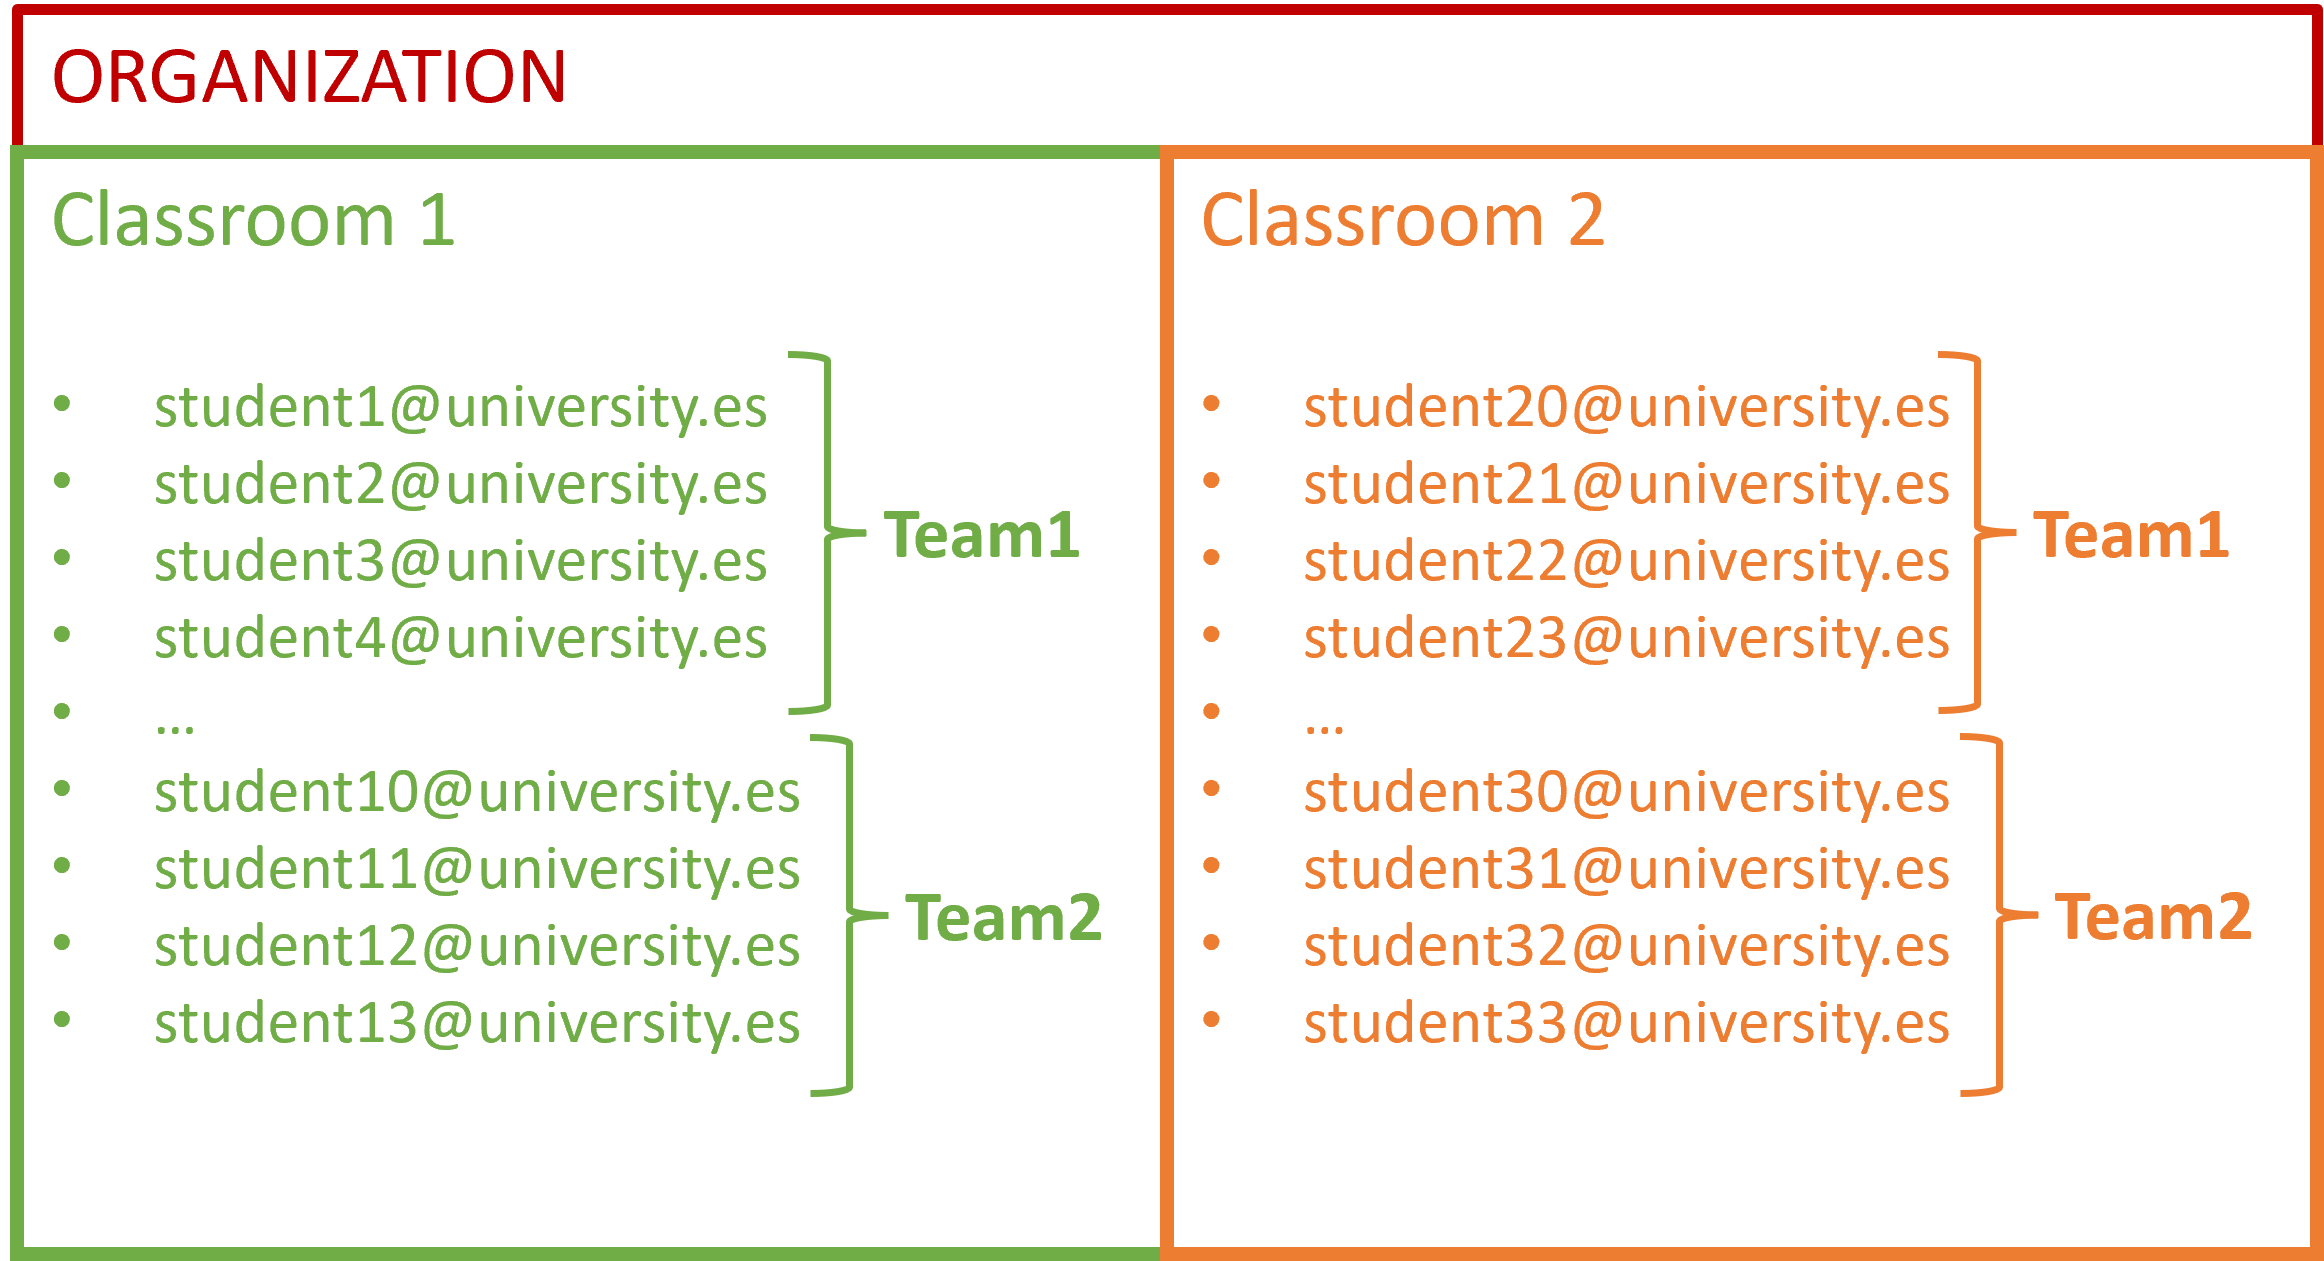
\includegraphics[width = \textwidth]{Figures/OrgGHClass.png}
    \caption{Basic structure for grouping students with GitHub Classroom.}
    \label{fig:OrgGHClass}
\end{figure} 


An assignment, whether it is individual or for groups, can be public or private, this option must be selected while creating the assignment. 
Notice that a public assignment allows students to see other classmates/groups work. 
In addition, an optional starter repository could be included to guide the students. 

Once the assignment is created, the available link should be shared with all the students so they can accept the invitation for the assignment and start working.  
Then, for each student or team that accepts the invitation, a copy of the template repository is made for each student or group. 
A list of accepted assignments is available for the teacher so the progress of each one can be tracked. Furthermore, a chat is opened between the teacher and the student 
to facilitate the communication, share comments, ask questions or feedback, etc. 















%
%\section{How to collaborate using Git + GitHub}
%
%
%\newpage 
%
%The following work flow applies both for the owner of the repository or for the collaborator.
%\begin{enumerate}
%\setlength\itemsep{0.0cm}
%    \item Create a branch based on the master branch. Identify that branch with a succint label describing the 
%    specific task or modification  to do.
%    \item Make changes on that branch. 
%    \item Commit those changes. 
%    \item Push to GitHub repository your changes. 
%    \item Pull request to merge your modifications with the master branch. 
%    \item Create the pull request and solve possible conflicts with the master branch. 
%    \item Merge the accepted changes with the master branch. 
%\end{enumerate}
%
%
%\begin{itemize}
%\setlength\itemsep{0.0cm}
%    \item Leave the branch "main" for the final product that we could give to the students, must be compiling and working.
%    \item Each time someone starts a task creates a branch from GH or GH Desktop. Even if it is revising the text and correcting one comma. 
%    \item When the task is finished creates a Pull Request in Git Hub with explanation of the changes.
%    \item Manages the possible conflicts when it is pulled (together we can do this step is necessary).
%    \item After that, the branch is deleted in Git Hub.
%    \item And deleted from the local GH Desktop (not to confuse next time modifying something THAT HAS NOT THE MOST UPDATED branch main).
%    \item Finally someone deletes the .pdf in the main branch because it only has the information of the last pulled in the history, and 
%specifically compiles and creates a new .pdf with all the state of the main branch, then the pdf is fully accordant to the main.
%    
%\end{itemize}
%
%
%Once you have the repository cloned in your local storage and you want to start working:
%
%\begin{enumerate}
%
%
%    \item Fetch and Pull the Master branch so you start with the most recent state of the project.
%    \item Create a new branch based on the main branch, name it according to the task you are going to perform.
%    
%    
%    
%    \item Work on that branch, make commits, push those commits to store everything in GitHub and create issues to ask for help to your 
%    collaborators. 
%    Remember that the longer you work on a branch without merging with the master one, the more probable it will be for conflicts to appear 
%when merging.
%    \item Once finished, if you have a final product that works, to merge in the master branch create a pull request with the latest changes.
%    \item Validate all the changes with your collaborators.
%    \item Merge the branch into the master branch.
%    \item Delete th branch (locally and remotely), this one does not have the changes made by the collaborators while you were working.
%    \item Fetch and Pull the Master branch in your local repository and start again. 
%\end{enumerate}
%
%
%
%
%
%
%
%
%
%
%
%
%
%
%
%
%
%
%\section{Create GitHUB repository from local project}
%
%Committing and pushing are how you can add the changes you made on your local machine to the remote repository in GitHub. That way your 
%instructor and/or teammates can see your latest work when you’re ready to share it. You can make a commit when you have made changes to your 
%project that you want to “checkpoint.” You can also add a helpful commit message to remind yourself or your teammates what work you did 
%(e.g. 
%“Added a README with information about our project”).
%
%Once you have a commit or multiple commits that you’re ready to add to your repository, you can use the push command to add those changes to 
%your remote repository. Committing and pushing may feel new at first, but we promise you’ll get used to it 🙂
%
%
%
%\begin{itemize}
%\item COMMIT.
% 
%\item PUSH
%\item PULL
%\item FETCH
%\item PULL REQUEST
%\item MERGE 
%\item REBASE
%\item FORKS
%\end{itemize} 
%
%
%
%
%
%
%%------------------------------------------------------------------------------------------------------
%\section{Creating a GitHub repository}
%   
%The main characters in the VCS explained in this chapter are the following, 
%consider which of them can be useful for your situation.  
%
%\begin{itemize}
%    \item Git 
%    \item GitHub account
%    \item GitHub Extension for Visual Studio, GitHub Desktop or both
%    \item GitHub Classroom account
%\end{itemize}
%   
%First of all, in order to use all the tools mentioned here, get sure that you already have a GitHub account, whether it is personal or with 
%your institutional email. If GitHub classroom is going to be used it is recommended the institutional email. 
%    
%To install Git an executable installer can be freely obtained from its main website: \underline{https://git-scm.com/}. Look for your 
%operating system and download the installer, then install it in your computer by following the steps. Another option is to install Git from 
%the Visual Studio installer; open and update it, go to Individual Components tab and find ``GIT for Windows'', select it and click on 
%``Modify''. Both ways install the tool for your computer, independently of using it with Visual Studio, a different IDE or the command 
%prompt.
%
%Once finished, by opening a command line you should be able to execute a git command, for example type: \texttt{git help git} on your 
%command 
%window, the Manual page should open in your browser. Now, git is available in your computer and it can be used in many different projects 
%like \LaTeX documents, Visual Studio solutions (\texttt{.sln}), MATLAB projects, etc. 
%
%In order to fully use GitHub integrated with all the projects mentioned before different options are available:
%
%\begin{enumerate}
%    \item If you are using Visual Studio install the GitHub extension in the IDE. Open EXTENSIONS and click on ``Manage Extensions'', open 
%    the tab ``Online'', look for the GitHub tool and install it. 
%    \item If your IDE does not have a GitHub integrated tool you can also manage it with GitHub Desktop, an application that brings and 
%    extents the potential of GitHub independently of the IDE used or the project being developed. 
%\end{enumerate}


%Crear Git repository o clonar uno existente
%Ya sea local o remoto
%Flujo de trabajo en ambas herramientas
%gitignore es LO PRIMERO QUE HAY QUE CREAR y readme creo que tambien


%\newpage 



    
%    \section{Create a Git repository of a solution}
%
%To add a Git repository to the solution proceed with the following steps:
%
%\begin{enumerate}
%    \item Open your version of Visual Studio.
%    \item Open the solution.
%    \item In the solution explorer, right click on the name of your solution and select \textit{Add Solution to Source Control...} (Figure \ref{fig:Git0}).
%    \item Click on \textit{View/Team Explorer} and check that the repository has been created (Figure \ref{fig:Git1}).
%\end{enumerate}
%
%\begin{figure}[h]
%    \centering
%    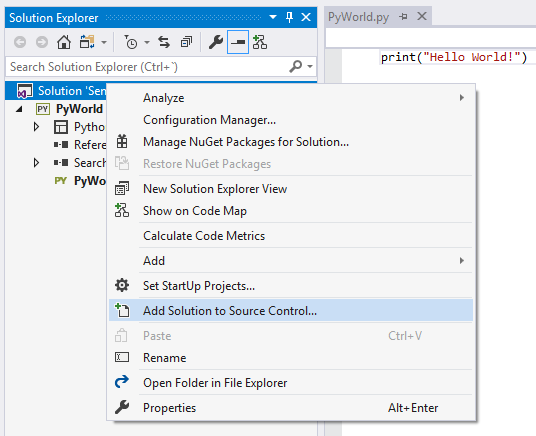
\includegraphics[width=0.7 \textwidth]{Figures/G0V1.png}
%    \caption{Adding Version Control to an existing Visual Studio solution.}
%    \label{fig:Git0}
%\end{figure}
%
%\begin{figure}[h]
%    \centering
%    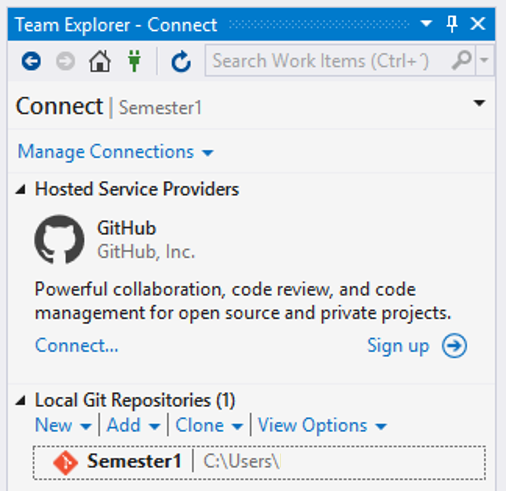
\includegraphics[width=0.5 \textwidth]{Figures/G1V2.png}
%    \caption{\textit{Team Viewer} tab. The solutions with Git repositories are shown in the \textit{Local GIT repositories} menu.}
%    \label{fig:Git1}
%\end{figure}
%
%%\begin{figure}[h]
%%\centering
%%\caption{New Git repo.}
%%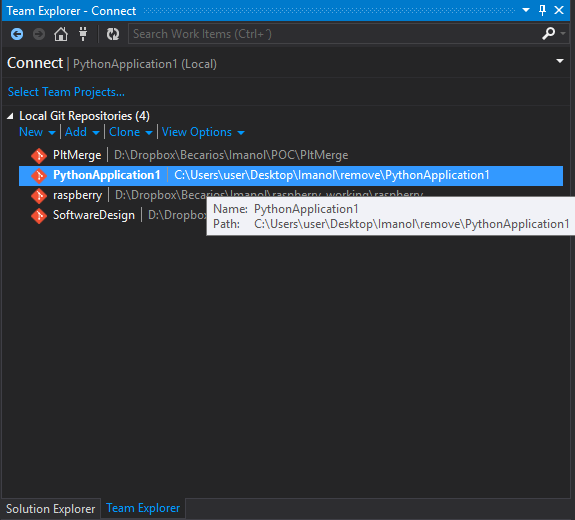
\includegraphics[width=0.85 \textwidth]{Figures/git2.PNG}
%%\label{fig:Git2}
%%\end{figure}
%
%    \section{Save changes on a Git repository}
%
%While developing a software project a large number of files are modified, renamed and deleted. Periodically we want to save all the changes performed in a work session by updating the repository. In order to do that, follow these steps:
%
%\begin{enumerate}
%    \item Open an existing Visual Studio solution with a Git repository.
%    \item Click on \textit{View/Team Explorer} or on \textit{Team Viewer} tab.
%    \item Click on the \textit{Home} icon (
\includegraphics[height=11pt]{./Figures/Home.png}).
%    \item Click on \textit{Changes}.
%    \item Write a short comment on the text area (Figure \ref{fig:GitCommit0}).
%    \item Click on \textbf{confirm all}.
%\end{enumerate}
%
%\begin{figure}[h]
%    \centering
%    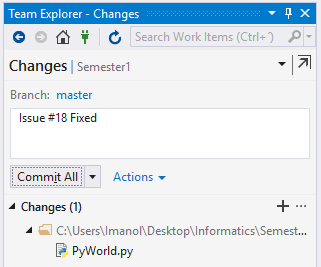
\includegraphics[width=0.5 \textwidth]{Figures/GCV2.png}
%    \caption{\textit{Changes} section of the \textit{Team Viewer} tab. In this case the script \textit{PyWorld.py} has changed since the last version updated and it is going to be saved again.}
%    \label{fig:GitCommit0}
%\end{figure}
%
%
%
%
%    \section{Configure GitHub}
%
%If we have already installed the GitHub extension we can configure our account. The following steps describe how to upload our projects to the web with the GitHub account:
%
%\begin{enumerate}
%	\item Open Visual Studio.
%	\item Open an existing solution with a Git repository.
%	\item On \textit{View/Team Explorer} and click on the \textit{Home} icon.
%	\item Click on \textit{Sync}.
%	\item In the \textit{Publish to GitHub} section, click on \textit{Sign in} in order to log in with your account (Figure \ref{fig:GitHub0}).
%	\item Push the repository to GitHub (Figure \ref{fig:GitHub2}).
%\end{enumerate}
%
%\begin{figure}[h]
%	\centering
%	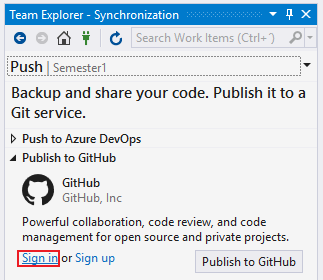
\includegraphics[width=0.5\textwidth]{Figures/GH0V3.png}
%	\caption{\textit{Sync} tab of the Team Viewer. Git repositories can be published on remote servers such as \textit{Team Services} or \textit{GitHub}.}
%	\label{fig:GitHub0}
%\end{figure}
%
%%\begin{figure}[h]
%%	\centering
%%	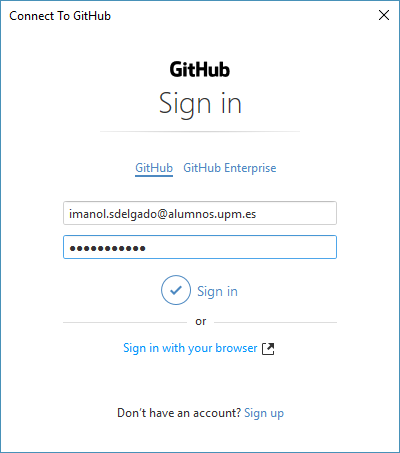
\includegraphics[width=0.4\textwidth]{Figures/GH1.png}
%%	\caption{GitHub Sign in window.}
%%	\label{fig:GitHub1}
%%\end{figure}
%
%\begin{figure}[h]
%	\centering
%	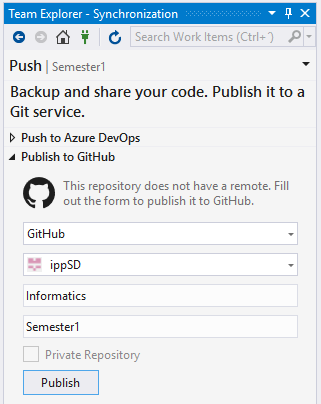
\includegraphics[width=0.5\textwidth]{Figures/GH2V3.png}
%	\caption{\textit{Sync} tab in the Team Viewer. If we have a \textit{GitHub} account we can publish our Git repositories.}
%	\label{fig:GitHub2}
%\end{figure}
%
%    \section{Import projects from GitHub}
%
%Visual Studio can create solutions from the source code of remote repositories obtained from GitHub thanks to the extension installed in the previous sections. In order to import a repository follow this:
%
%\begin{enumerate}
%	\item Go to \textit{View/Team Explorer} as usual.
%	\item Click on the \textit{Manage Connections} icon (
\includegraphics[height=11pt]{./Figures/Connect.png}).
%	\item In the \textit{GitHub} section select \textit{clone}.
%	\item Select a \textit{Repository name} (Figure \ref{fig:GitHubClone1}).
%	\item Select a \textit{path} for saving the repository.
%	\item Click on \textit{Clone}.
%	\item Go to the \textit{Team Viewer} tab and click on \textit{Manage Connections} icon once again (Figure \ref{fig:GitHubClone2}).
%	\item Double click on the downloaded \textit{Repository name}.
%	\item If there is no solution on the \textit{Solutions} section, select \textit{New...} in order to create it.
%	\item Create a solution for the repository according to the programming language of the source code.
%\end{enumerate}
%
%\begin{figure}[H]
%	\centering
%	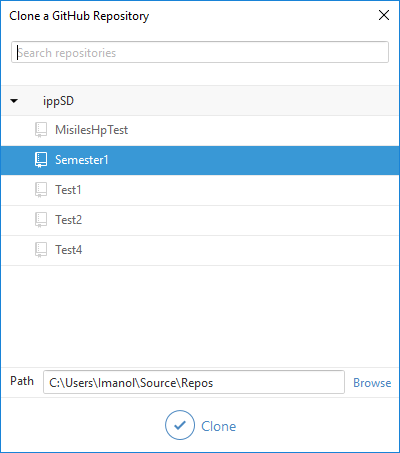
\includegraphics[width=0.5\textwidth]{Figures/GHC1.png}
%	\caption{Available Git repositories list on a GitHub account that can be cloned by Visual Studio.}
%	\label{fig:GitHubClone1}
%\end{figure}
%
%\begin{figure}[H]
%	\centering
%	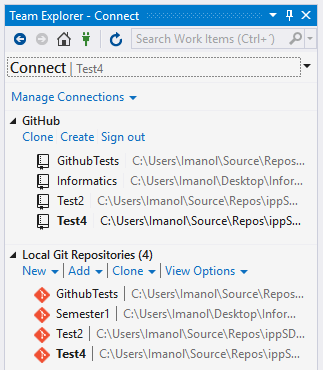
\includegraphics[width= 0.5\textwidth]{Figures/GHC3V3.png}
%	\caption{Available local Git repositories.}
%	\label{fig:GitHubClone2}
%\end{figure}
%
%    \section{Download repository updates from GitHub}
%
%While working as a team, it is possible that two or more people make changes on the remote repository at the same moment. These changes must be \textbf{pulled} from GitHub in order to have an updated version of the code and make sure that all members work on the same source files. In order to check the updates, follow the next steps:
%
%\begin{enumerate}
%	\item Go to \textit{View/Team Explorer} and click on the \textit{Home} icon.
%	\item Click on \textit{Sync}.
%	\item Select \textit{Recover} in order to getting the changes from the remote repository.
%	\item Click on \textit{Extract} for applying those changes.
%\end{enumerate}
%
%    \section{Upload local changes to GitHub}
%
%Once our project is ready, it has to be \textbf{pushed} to the remote repository so that every team member has access to the last updates. This can be made by following these steps:
%
%\begin{enumerate}
%	\item Commit changes of the current project.
%	\item Go to \textit{View/Team Explorer} (or the \textit{Team Viewer} tab) and click on the \textit{Home} icon.
%	\item Click on \textit{Sync}.
%	\item Click on \textit{sync} for automatically synchronize all commits.
%\end{enumerate}
%
%    \section{Avoid uploading specific files to the repository}
%
%When saving changes to the Git repository, all files generated by the project such as compiled, temporary or output files are included. We might not want all of them to be uploaded, just source code and documentation for example. Git includes a configuration file, \textbf{gitignore}, where the files and folders to be skipped are recorded. In order to edit this file follow the next steps:
%
%\begin{enumerate}
%	\item Open a Git configured Visual Studio solution.
%	\item Go to \textit{Team Viewer} tab and click on the \textit{Home} icon.
%	\item Click on the \textit{Settings} button and select \textit{Repository Settings}.
%	\item Unfold the \textit{Ignore \& Attributes Files} menu and click on the \textit{Edit} link next to \textit{Ignore File} (Figure \ref{fig:GitIgnore0}).
%	\item Edit the \textit{gitignore} file.
%\end{enumerate}
%
%\begin{figure}[h]
%	\centering
%	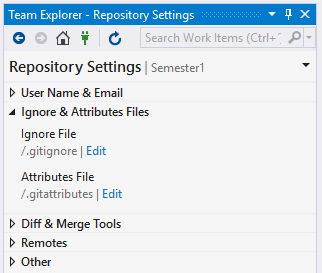
\includegraphics[width= 0.7\textwidth]{Figures/GIG0.png}
%	\caption{Menu for accessing the Gitignore file.}
%	\label{fig:GitIgnore0}
%\end{figure}
%
%\textit{gitignore} uses \textit{Regex} (Regular Expressions) syntax for selecting files. Figure \ref{fig:GitIgnore1} shows an example with the most common expressions:
%
%\begin{itemize}
%	\item All lines: text placed after the hash symbol (\#) are comments with no real effect.
%	\item Line 266: asterisk (*) matches any text. In this case, files ending with \textit{pyc} extensions are omitted.
%	\item Line 268: double asterisk (**) matches any folder. In this case, the \textit{\_\_pycache\_\_} folder is omitted on all subdirectories of the repository.
%	\item Lines 273, 274: Regex syntax can be used multiple times on the same line. In these cases, folders containing \textit{Advisor} or \textit{OLD} are omitted from all subdirectories of the repository.
%	\item Line 272: Characters inside square brackets ([...]) are used for text combinations. In these cases, \textit{Debug}, \textit{debug}, \textit{DebugPublic}, \textit{debugPublic} folders are omitted.
%\end{itemize}
%
%\begin{figure}[h]
%	\centering
%	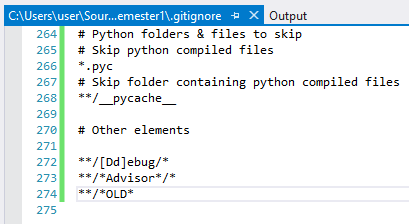
\includegraphics[width= 0.8\textwidth]{Figures/GIG1.png}
%	\caption{Gitignore example.}
%	\label{fig:GitIgnore1}
%\end{figure}
%
%    \section{Git and GitHub FAQ}
%
%\begin{itemize}
%    
%    %%%%%%%%%%%%%%%%%%%%%%%%%%%%%%%%%%%%%%%%%%%%%%%%%%%%%%%%%%%%%%%%%%%%%%%%%%%%%%%%%%%%%%%%%%%%%%%
%	\item \textbf{I can not save changes on GitHub: Updates were rejected because the remote contains work that you do not have locally}.
%	
%	This occurs because there were changes on the remote repository that you did not updated. Since you have modified outdated files, now there are conflicts on the files and it has to be solved manually. You have to download them first and then upload the new code:
%	
%	\begin{enumerate}  
%		\item Go to \textit{Team Viewer} tab and click on the \textit{Home} icon.
%		\item Click on \textit{Sync}.
%		\item Click on \textit{Recover}. The new changes should appear.
%		\item Click on \textit{sync}.
%		\item There might be errors on merging (Figure \ref{fig:GitHubErr1}).
%		\item Click on \textit{Conflicts}.
%		\item Select a \textit{conflict file}.
%		\item There are several ways of solving conflicts (Figure \ref{fig:GitHubErr2}):
%		\begin{enumerate}
%			\item \textit{Take remote} file and discard local changes.
%			\item \textit{Keep local changes} and override remote file.
%			\item \textit{Merge by combination} both files and select code to be kept and discard.
%		\end{enumerate}
%    	\item Sync again.
%        %\begin{figure}[h]
%        %	\centering
%        %	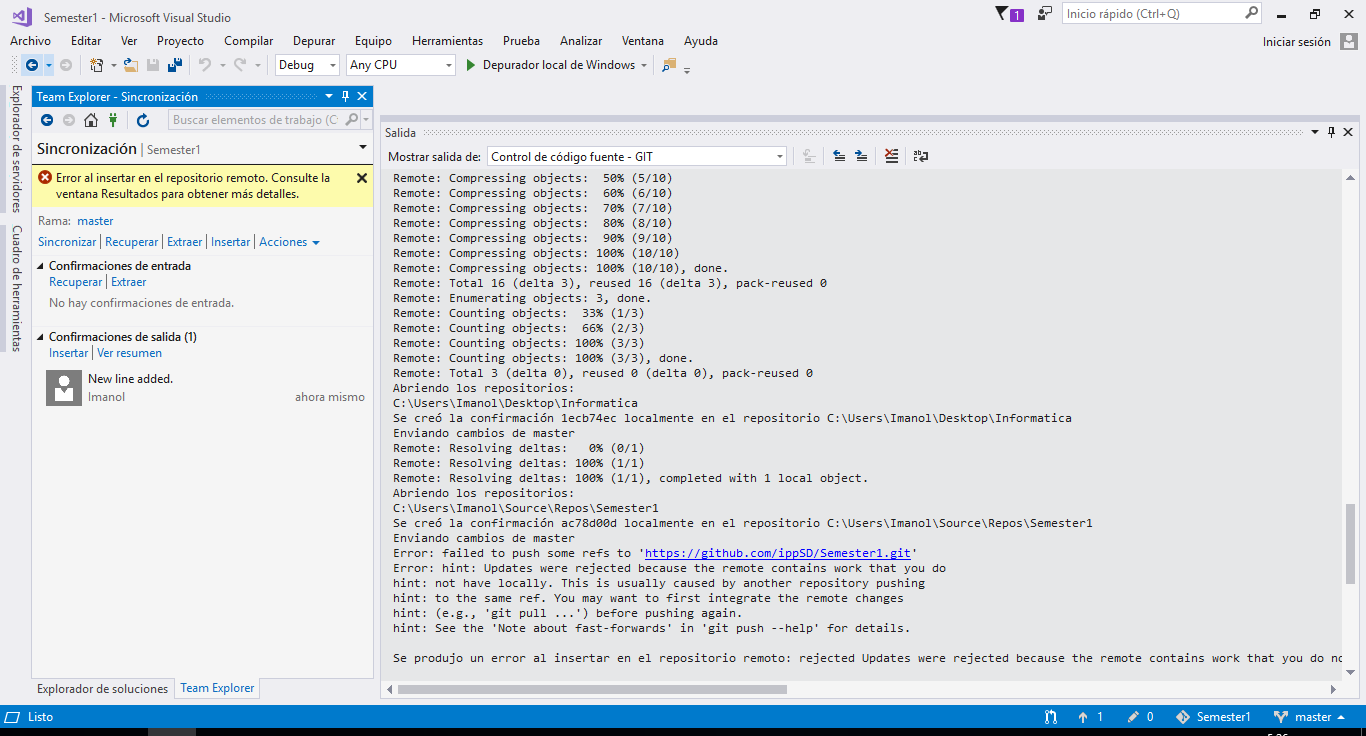
\includegraphics[width=\textwidth]{Figures/GHERR0.png}
%        %	\caption{Common Git error o}
%        %	\label{fig:GitHubErr0}
%        %\end{figure}
%        
%        \begin{figure}[h]
%        	\centering
%        	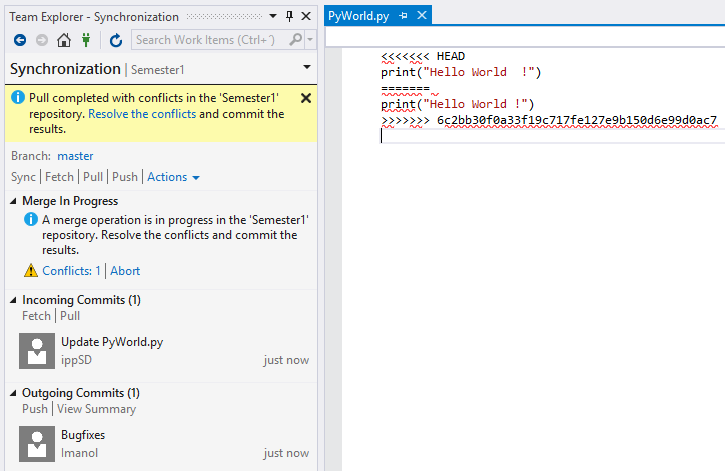
\includegraphics[width=\textwidth]{Figures/GHERR1V1.png}
%        	\caption{Solving conflicts with local and remote repositories, step 1.}
%        	\label{fig:GitHubErr1}
%        \end{figure}
%        
%        \begin{figure}[h]
%        	\centering
%        	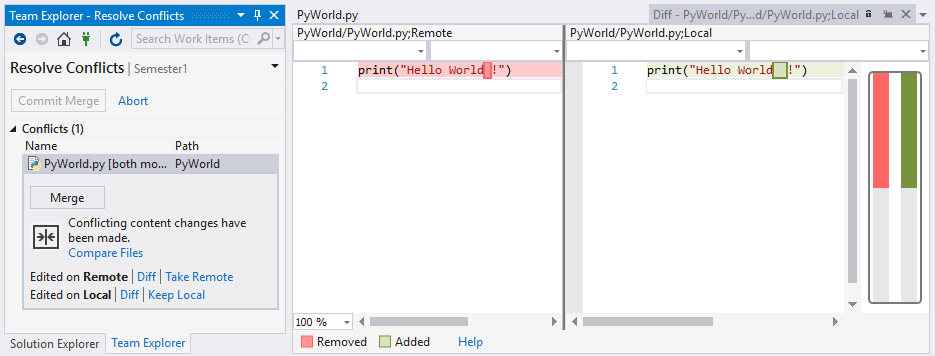
\includegraphics[width=\textwidth]{Figures/GHERR2V1.png}
%        	\caption{Solving conflicts with local and remote repositories, step 2.}
%        	\label{fig:GitHubErr2}
%        \end{figure}	
%	\end{enumerate}
%	
%    %%%%%%%%%%%%%%%%%%%%%%%%%%%%%%%%%%%%%%%%%%%%%%%%%%%%%%%%%%%%%%%%%%%%%%%%%%%%%%%%%%%%%%%%%%%%%%%
%	\item \textbf{How can I unbind a project from GitHub?}
%	
%	A local Git repository can be unlinked from the remote repository on the configuration settings:
%	
%	\begin{itemize}
%		\item Go to \textit{Team Viewer} tab as usual and click on the \textit{Home} icon.
%		\item Click on \textit{Configuration}.
%		\item Click on \textit{Repository Configuration}.
%		\item In the \textit{remote} section, click on \textit{remove}.
%	\end{itemize}
%
%    %%%%%%%%%%%%%%%%%%%%%%%%%%%%%%%%%%%%%%%%%%%%%%%%%%%%%%%%%%%%%%%%%%%%%%%%%%%%%%%%%%%%%%%%%%%%%%%
%	\item \textbf{I changed the \textit{gitignore} file but the omitted files are still being uploaded}
%	
%	This occurs when the files/folders to be omitted where first saved in the repository and then included on the \textit{gitignore} file. In order to fix this issue, a quick workaround is made:
%	
%	\begin{enumerate}
%		\item Save changes to the git repository. This commit will serve as a backup.
%		\item Move all the files/folders you want to omit out of the solution directory.
%		\item Save the new changes to the git repository. Displaced files will be removed from the repository.
%		\item Restore the moved files/folders on their original directories.
%		\item Save the new changes to the git repository. Due to omitted files being removed and \textit{gitignore} blocking them these files will not appear again.
%	\end{enumerate}
%
%
%    %%%%%%%%%%%%%%%%%%%%%%%%%%%%%%%%%%%%%%%%%%%%%%%%%%%%%%%%%%%%%%%%%%%%%%%%%%%%%%%%%%%%%%%%%%%%%%%
%	\item \textbf{How can I upload files to GitHub without Visual Studio?}
%		
%	Source code, graphics, documentation, etc. can be uploaded to GitHub without using the \textit{Team Viewer} window by using either \textbf{Git Command Line Tools} or the \textbf{GitHub Web Page}. Since command line tools require additional software, only the web approach will be explained. 
%		
%%		\subsubsection*{\textbf{Git Command Line Tools}}
%%		
%%		\begin{enumerate}
%%			\item Right click on \textit{??}.
%%			\item Place files and folders on said folder.
%%			\item Add and commit new files to the repository:
%%\begin{lstlisting}
%%$ git add *
%%$ git commit -m "COMMIT MESSAGE"\end{lstlisting}
%%			\item Add your remote repository location, \textit{REPOSITORY-URL}. The remote address will be aliased as \textit{origin}.
%%\begin{lstlisting}
%%$ git remote add origin "REPOSITORY-URL" \end{lstlisting}
%%			\item Push changes to GitHub:
%%\begin{lstlisting}{bash}
%%$ git push -u origin master\end{lstlisting}
%%		\end{enumerate}
%		
%    %\subsubsection*{\textbf{GitHub Web Page}}
%    
%    Files and folder can be easily saved by dropping them onto the web browser.
%    
%    \begin{enumerate}
%    	\item Log in \textit{https://github.com} with your credentials.
%    	\item Open the GitHub repository page where files must be stored.
%    	\item On the \textit{Code} tab, click on \textit{Upload Files} button.
%    	\item Drag the files and folders onto the browser.
%    	\item \textit{Commit} changes before closing the web page. 	
%    \end{enumerate}	
%\end{itemize}
%
%\begin{figure}[h]
%	\centering
%	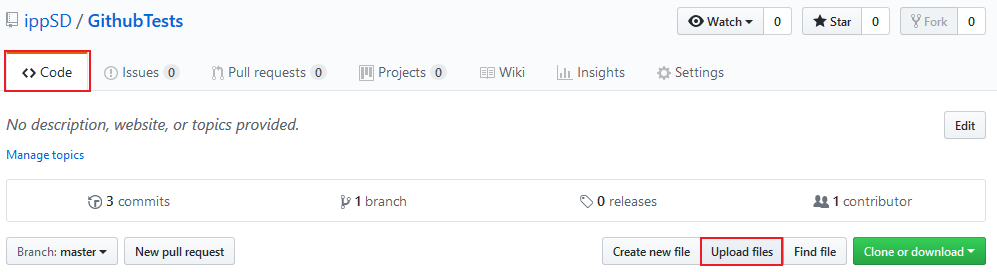
\includegraphics[width=\textwidth]{Figures/GUP0.png}
%	\caption{How to upload files to GitHub manually (first step).}
%	\label{fig:GitHubUpload0}
%\end{figure}
%
%\begin{figure}[h]
%	\centering
%	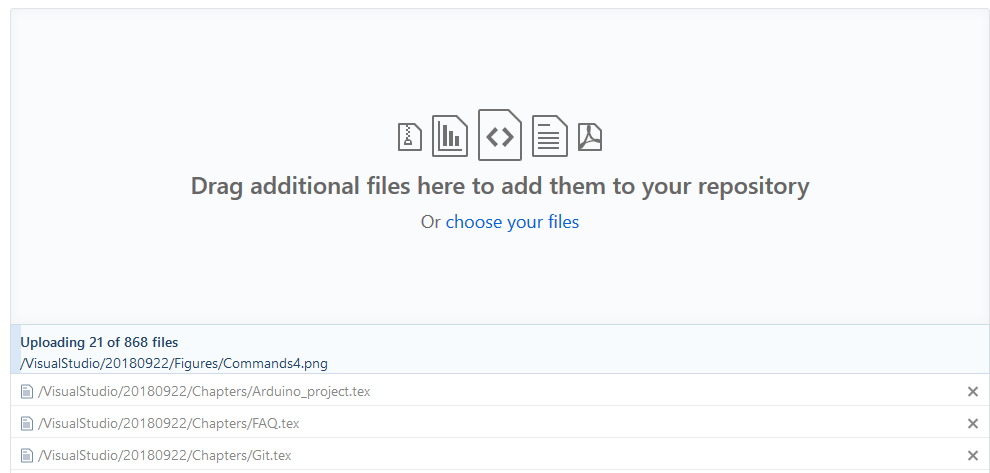
\includegraphics[width= \textwidth]{Figures/GUP1.png}
%	\caption{How to upload files to GitHub manually (second step).}
%	\label{fig:GitHubUpload1}
%\end{figure}
%
%\begin{figure}[h]
%	\centering
%	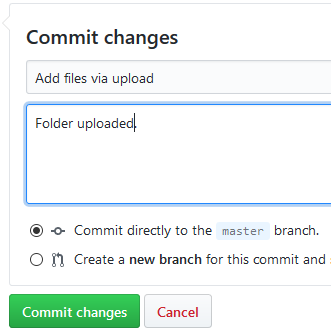
\includegraphics[width=0.5 \textwidth]{Figures/GUP2.png}
%	\caption{How to upload files to GitHub manually (third step).}
%	\label{fig:GitHubUpload2}
%\end{figure}



























%\clearpage
%\section{Visual Studio Git commands}
%
%When a project is selected on \textbf{Team Explorer} panel there are several 
%options available by expanding the top horizontal bar:
%
%\begin{itemize}
%\item \textbf{Changes}: includes the project saving commands.
%\item \textbf{Branches}: manages branches of the repository.
%\item \textbf{Unsynced Commits}: allows remote operations.
%\item \textbf{Settings}: Git settings.
%\end{itemize}
%
%\subsection{Bind Visual Studio to a person}
%
%On team working the username and email address is compulsory so it has to be 
%changed on Git Settings.
%
%\begin{enumerate}
%\item Set username and email:
%On \textbf{Team Explorer} panel and on your Git repository, Select on the top 
%horizontal bar \textbf{``Settings{$\rightarrow$}Git Settings''}. Add/change 
%\textbf{User Name} and \textbf{Email Address}, then press \textbf{Update}
%\end{enumerate}
%
%\subsection{Commit your code}
%
%\begin{enumerate}
%\item On \textbf{``Team Explorer''} panel, select your Git repository and go to 
%\textbf{``Changes''}.
%
%\item If you want to hide a file/folder from your repository (``OLD'' folders, 
%``*.bak'' files, etc.), on the \textbf{``Included Changes''} tree select your 
%folder/file and select \textbf{``Exclude''}.
%
%\item If you want to add a new version of an excluded folder/file, right click 
%and \textbf{``Include''} on the \textbf{``Excluded Changes''} tree.
%
%\item Set a \textbf{``commit message''} and hit the \textbf{``commit''} button.
%\ref{fig:Git3}
%
%
%\begin{figure}[h]
%\centering
%\caption{Git ``Changes'' option.}
%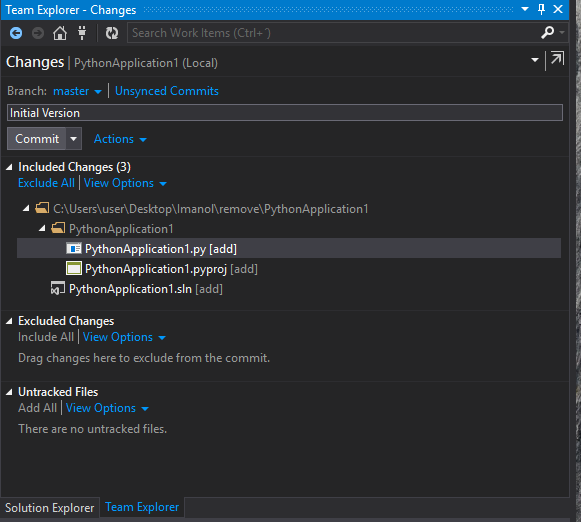
\includegraphics[scale=0.6]{Figures/git3.PNG}
%\label{fig:Git3}
%\end{figure}
%
%\end{enumerate}






%%%%%%%%%%%%%%%%%%%%%%%%%%%%%%%%%%%%%    OLD    %%%%%%%%%%%%%%%%%%%%%%%%%%%%%%%%%%%%%%%%%%%

% According to Visual Studio Documentation, VCS are defined in the following way:
%
%\begin{center}
%    \begin{minipage}{0.7\linewidth}
%        \vspace{5pt}        %margen superior de minipage
%        {\small
%            ``Version control systems help you track changes to code over time. 
%            As you make changes, the version control system takes a snapshot of 
%            your files. The version control system saves that snapshot 
%            permanently so you can recall it later if you need it...''
%        }
%        \begin{flushright}
%            (\url{https://docs.microsoft.com/en-us/visualstudio/version-control/?view=vs-2017})
%        \end{flushright}
%        \vspace{5pt}%margen inferior de la minipage
%    \end{minipage}
%\end{center}


%natively, Git included. For 
%an easy experience Visual Studio offers a simple GUI so that only a little 
%concepts are required.
%
%Git with Visual Studio can clone a remote project from GitHub, GitLab or even a 
%custom server in order to work as a team.

%\section{Git most important commands}
%
%This section explains the basic Git commands and provides a better 
%understanding of how to work on Git.
%
%\subsection*{Commands for creating a project}
%Initialization commands:
%
%\begin{itemize}
%\item \textbf{init}: create an empty Git repository.
%\item \textbf{clone}: download a Git repository from an URL or a local 
%directory.
%\end{itemize}
%
%\subsection*{Commands for saving a project}
%
%Once on a working Git repository, new created and modified files must be added 
%to a queue so that they are added to the repository when necessary. These are 
%the basic commands:
%
%\begin{itemize}
%\item \textbf{add}: add files and folders to your repository's changes queue. 
%Some will appear as new, others as modified and some even as renamed.
%\item \textbf{commit}: uploads the changes queue to the repository. Now the 
%changes have been submitted and the changes queue is empty.
%\end{itemize}
%
%\subsection*{Commands for making branches}
%
%Branches allow the user to separate ways from a common origin, which means that 
%changes on a branch will not affect to others. It is useful for having a 
%working and compiling project (e.j. \textit{master}) and a testing branch (e.j. 
%\textit{dev}) so that when the testing works it can be uploaded to the main 
%project.
%\begin{itemize}
%\item \textbf{branch}: create a new branch from another one, being 
%\textit{master} as the default branch, or destroy an existing one. It creates a 
%new branch but it does not use it, so use the \textit{checkout} command before 
%editing anything else.
%\item \textbf{checkout}: change the working branch.
%\item \textbf{merge}: combines branches.
%\end{itemize}
%
%\subsection*{Commands for remote repositories}
%
%\begin{itemize}
%\item \textbf{pull}: get a commit, branch, etc. from remote.
%\item \textbf{push}: upload commit, branch, etc. to remote.
%\end{itemize}






%    \FloatBarrier
%    \section{Installing GitHub Extension}
%
%Visual Studio includes a GitHub extension for saving Git repositories on-line on your account. In order to install the extension follow these steps:
%
%\begin{enumerate}
%	\item Click on \textit{Tools/Extensions and Updates...}
%	\item Click on the tab ``Online'' on the left part of the window and then search for ``GitHub Extension for Visual Studio'' (you can use the Search engine).
%    \item Download it (Figure \ref{fig:GitHubTest0}).
%	\item Close all Visual Studio windows and follow the instructions of the \textit{GitHub extension installer} program.
%    \item The process will finish automatically after clicking on \textit{Modify} in one of the steps.
%\end{enumerate}
%
%\begin{figure}[h]
%	\centering
%	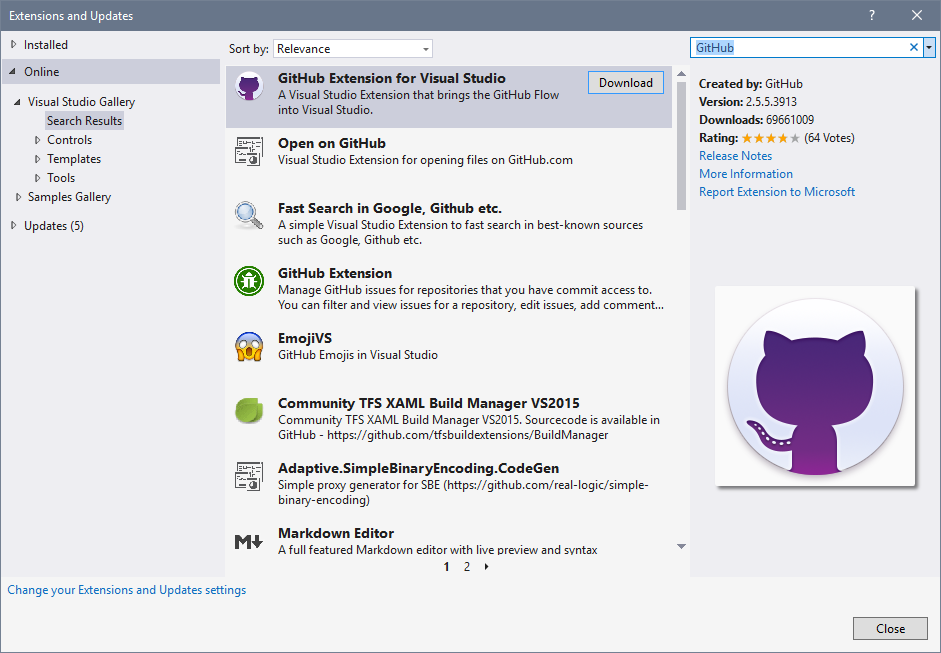
\includegraphics[width=\textwidth]{Figures/GH-1.png}
%	\caption{\textit{Extensions and updates} window of VS where the GitHub extension can be installed, updated or removed.}
%	\label{fig:GitHubTest0}
%\end{figure}\section{Create GitHUB repository from local project}
